\documentclass[]{book}
\usepackage[english]{babel}
\usepackage{graphicx}

\begin{document}


\chapter*{System}

\subsection*{Front-end electronics}
\noindent Según la configuración de los electrodos de recolección de carga del detector, es posible sensar eventos en varios canales de lectura paralelamente, logrando una importante resolución espacial. Sin embargo, en este trabajo se desarrolla un sistema monocanal para la adquisición de datos de un detector GEM como versión mínima funcional. Los electrodos de salida del detector están conectados en paralelo y conducidos a una única conexión con un cable tipo X. Posteriormente, se conecta una resistencia en serie para permitir la medición de la caída de voltaje en sus terminales, lo que convierte la señal de corriente original del detector en una señal de voltaje que puede ser acondicionada.\\

%inlcuir fotografía de los terminales soldados y la resistencia en serie con el conector del cable

En particular, el sistema de preamplificación utilizado en este trabajo es el Ortec 142B, un dispositivo charge-sensitive diseñado para capacitancias de entrada de entre 100 y 400 pF. %inlcuir fotografía del preamp\\
%qué tantas especificaciones técnicas del preamp debería incluir aquí?

La señal de salida del preamplificador está caracterizada por... y teniendo en cuenta que el ADC tiene un rango de trabajo de [citar satasheet del ADC500]..., es necesario agregar una etapa de amplificación para imprimir en la señal una ganancia de x.\\


%aquí seria necesario poner datos experimentales de la caracterización del detector, mostrando el factor de ganacia etc
%debería poner el desarrollo matemático de un charge-sensitive preamp? (lo tengo referenciado)

\noindent De esta manera, dando continuidad al recorrido de la señal después del preamplificador, se implementa un amplificador [referencia del amp NIM, ver page 812 Kolanoski], hacer una caracterización similar a la del preamp y preguntar si sacar curvas experimentales y qué tantos datos técnicos del fabricante. Terminar diciendo que ya la señal cuenta con las características adecuadas para ser digitalizada. \\

\noindent En este trabajo, se utilizó la tarjeta ICTP-INFN ADC500 como plataforma de digitalización, en adelante referida como ADC500 (véase fig \ref*{fig:adc500}). Esta tarjeta está basada en un Texas Instruments ADC08500 [4] de alta velocidad, con una frecuencia de muestreo de 500 MHz y 8 bits de resolución. Cumple con las especificaciones ANSI/VITA 57.1 y está equipada con un conector de tarjeta mezzanine FPGA (FMC) de bajo número de pines (LPC) [5].\\

\begin{figure}[h]
    \centering
    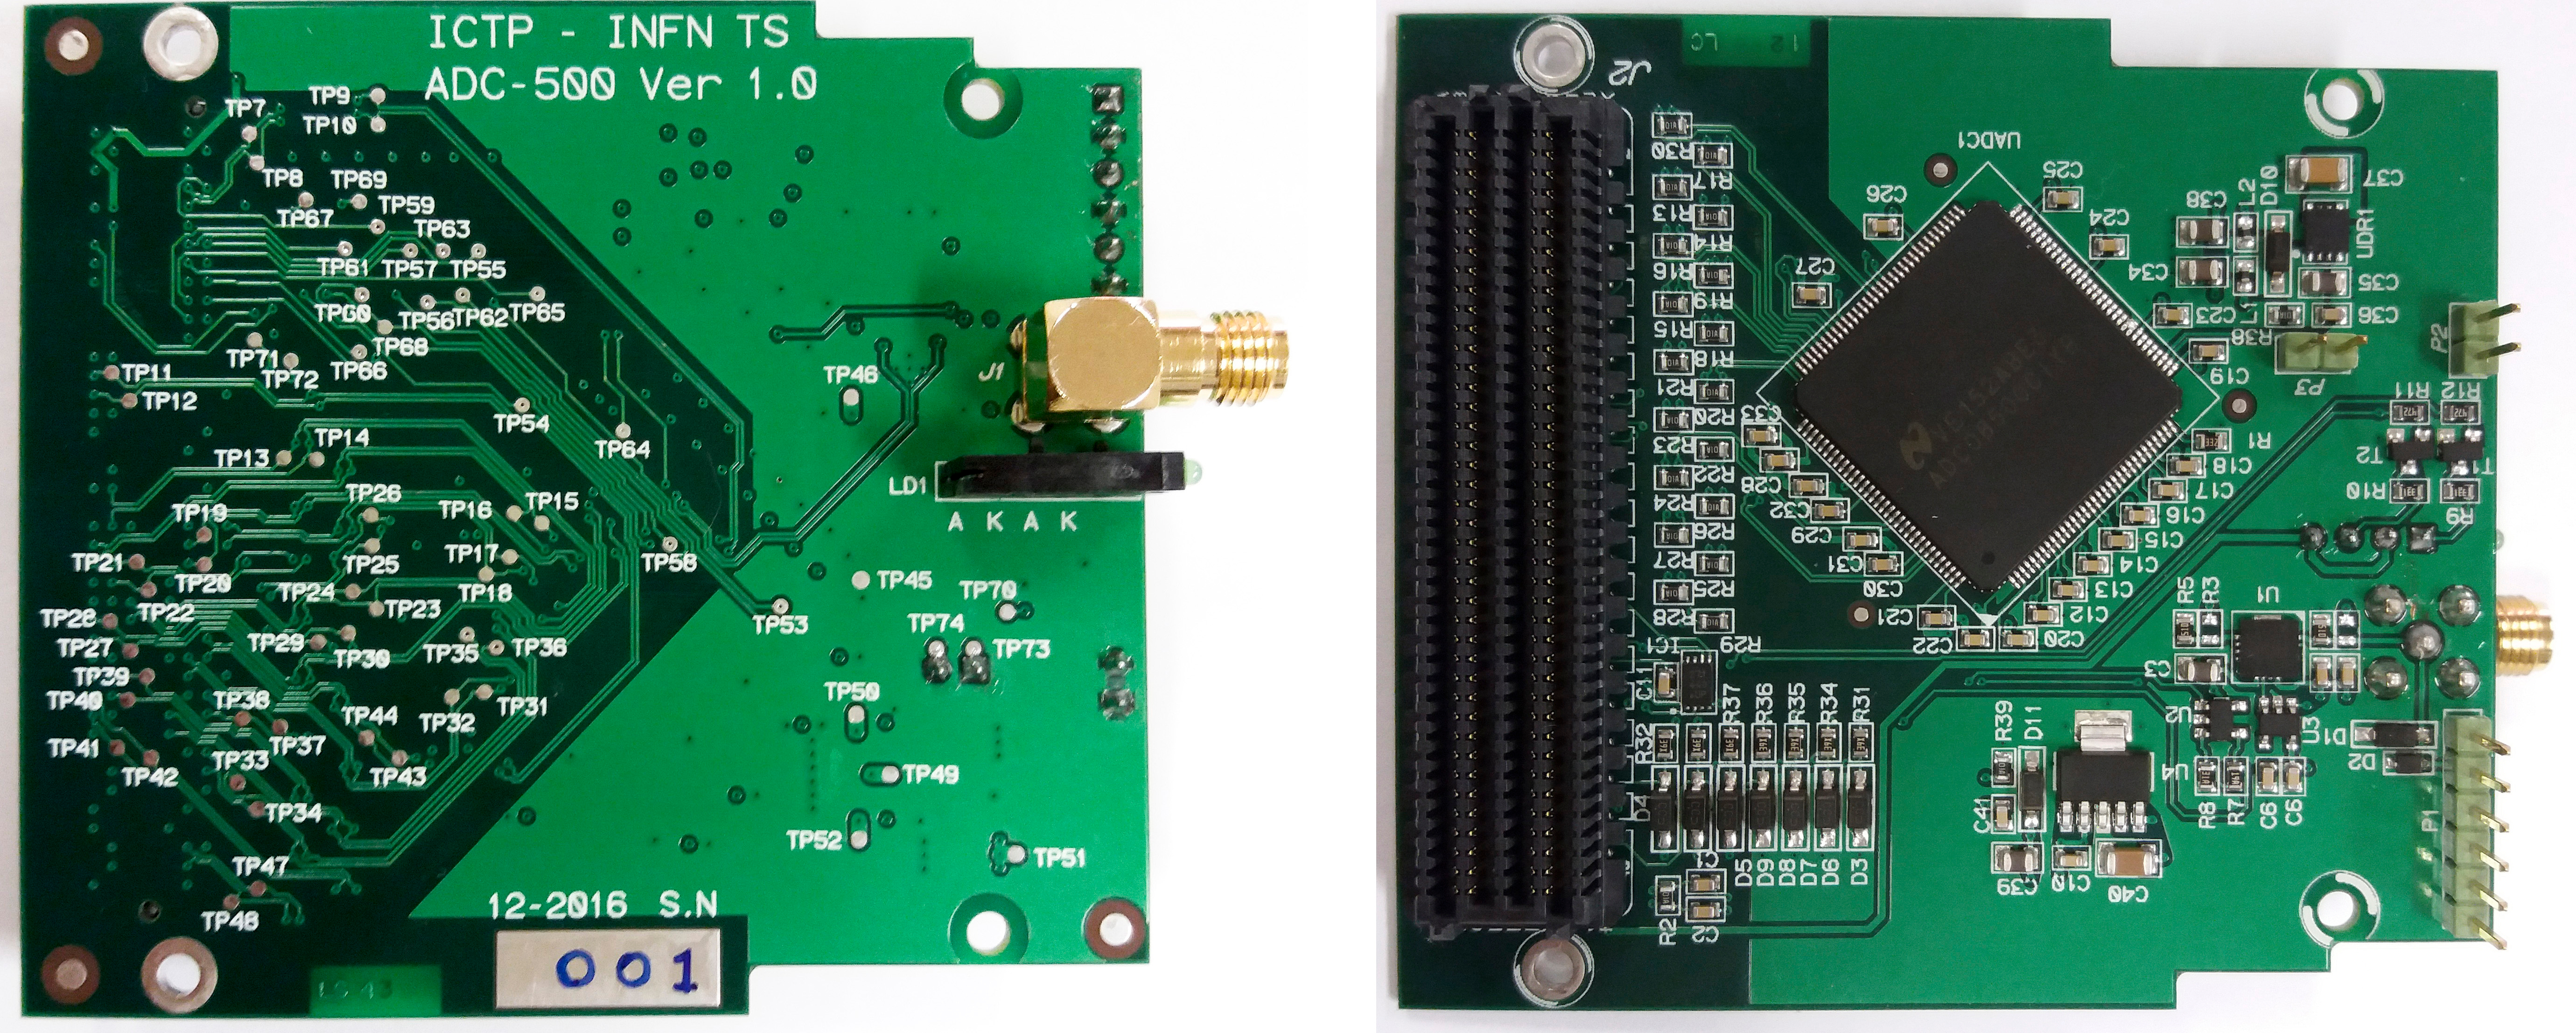
\includegraphics[width=0.8\textwidth]{ADC500.png}
    \caption{Plataforma de digitalización de señales ICTP-INFN ADC500. Tomada de [7].}
    \label{fig:adc500}

\end{figure}

\noindent Según el fabricante, el ADC cuenta con un demultiplexor 1:2 que alimenta dos buses de salida LVDS (Low-Voltage Differential Signaling). Los datos de estos buses se entregan a una tasa de palabras de salida en cada bus equivalente a la mitad de la tasa de muestreo del ADC, y deben ser intercalados por el usuario para proporcionar palabras de salida a la tasa de conversión completa. Esto implica que, una vez digitalizada la señal, esta es enviada mediante el protocolo LVDS a través del conector FMC hacia una plataforma digital compatible con las capacidades técnicas para realizar procesamiento paralelizado en tiempo real y a alta frecuencia. Para este fin,en este trabajo se propone el uso de la tarjeta de desarrollo Avnet Digilent Zedboard, que se basa en un SoC (System on Chip) Xilinx Zynq-7000, compuesto por una FPGA Artix-7 y un procesador ARM Cortex-A9 [6].

\end{document}